\section{Ejercicio 1}

\subsection{Introducción}

\paragraph{}
El primer problema del presente trabajo consistió en la implementación de un algoritmo capaz de dar solución a la ecuación 
	\begin{equation} 
		b^n\ mod\ (n)
	\label{problema}
	\end{equation}
haciendo uso de alguna de las técnicas algorítmicas aprendidas hasta el momento en la materia. Asímismo, la consigna dictaba que la complejidad final del algoritmo debería ser menor a \Ode{n}.

\paragraph{}
En pos de cumplimentar lo pedido se decidió usar la técnica de \textit{Dividir \& Conquistar}\footnote{Poner alguna referencia 	en donde se explique esta técnica} para desarrollar el algoritmo. Esta técnica se caracteriza principalmente en dividir la instancia de un problema en instancias más pequeñas, atacar cada una de ellas por separado y resolverlas, para finalmente juntar sus resultados y así producir el resultado final.


\subsection{Explicación}

\paragraph{}
La primera solución que se piensa casi de manera intuitiva para el problema es la de mutliplicar \textit{n} veces el número \textit{b} y luego hallar el resto de dividir ese resultado por \textit{n}. 
	\begin{equation}
		\underbrace{b.b.b \hdots b.b.b}_{n\ veces}\ mod\ (n)  = b^n\ mod\ (n)
	\label{primera_idea}		
	\end{equation}
Sin embargo, salta a la vista que la complejidad ese algoritmo es \Ode{n}, ya que se realizan \textit{n} multipicaciones y 1 división, razón por lo cual no cumple con lo pedido en la consigna. Además, puesto que ese algoritmo realizar sucesivas multipliciones de \textit{b}, cabe la posibilidad de que el valor que se va acumulando sobrepase el máximo número entero representable en la computadora produciedo así un overflow y obteniéndose en consecuencia un resultado incorrecto.

\paragraph{}
Analizando la falla del algoritmo anterior, se observa que lo que se debe evitar es calcular directamente el resultado de $b^n$ ya que ese número podría ser excesivamente grande. \\
Con esto en mente veamos una manera más conveniente de abordar el problema. Es claro, por definición de congruencia, que resover la ecuación en (\ref{problema}) equivale a hallar el \textit{x} tal que:
	\begin{equation}
		b^n\ \equiv\ x\ (n)\ , \hspace{10pt}\ con\ 0\ \leq\ x\ <\ n 
	\label{problema2}
	\end{equation}

Luego, asumamos por un momento que podemos tener gratis un k tal que:
	\begin{equation}
		b^{n/2}\ \equiv\ k\ (n)\ , \hspace{10pt}\ con\ 0\ \leq\ k\ <\ n 
	\label{divide}
	\end{equation}

Entonces, aplicando el resultado de (\ref{divide}) en (\ref{problema2}) obtenemos que:
	\begin{itemize}
		\item{
		Si \textit{n} es par:
			\begin{eqnarray}
				b^n\ \equiv\ x\ (n)\ , \hspace{10pt}\ con\ 0\ \leq\ x\ <\ n \nonumber\\
				b^{n/2}.b^{n/2}\ \equiv\ x\ (n) \nonumber\\
				k.k\ \equiv\ x\ (n) \nonumber\\
				k^2\ \equiv\ x\ (n)
			\label{recursion_par}
			\end{eqnarray}
		}
		
		\item{
		Si \textit{n} es impar par:
			\begin{eqnarray}
				b^n\ \equiv\ x\ (n)\ , \hspace{10pt}\ con\ 0\ \leq\ x\ <\ n \nonumber\\
				b.b^{n/2}.b^{n/2}\ \equiv\ x\ (n) \nonumber\\
				b.k.k\ \equiv\ x\ (n) \nonumber\\
				b.k^2\ \equiv\ x\ (n)
			\label{recursion_impar} 
			\end{eqnarray}
		}
	\end{itemize}
Luego, las expresiones resultantes en ambos casos pueden resolver de manera más simple y rápida ya que al estar acotado \textit{k} por \textit{n} el valor de $b.k^2$ es mucho menor que el de  $b^n$ y en consecuencia la operación de calcular el resto módulo \textit{n} se realiza en menor tiempo.

\paragraph{}
Volviendo un poco sobre nuestro pasos, se dijo anteriormente en (\ref{divide}) que podíamos asumir que obtener $k$ no tenía un costo computacional significativo. No obstante, esto no siempre es cierto puesto que para obtener \textit{k} es necesario calcular previamente $b^{n/2}$ el cual puede ser un número nada despreciable en lo que respecta a tamaño en memoria.\\
Si ese fuera el caso, entonces para calcular $b^{n/2}$ podemos aplicar nuevamente el procedimiento descripto con anterioridad calculando $b^{n/4}$ y usando una expresion análoga a (\ref{recursion_par}) o a (\ref{recursion_impar}) dependiendo de si $n/2$ es par o impar respectivamente. Del mismo modo se puede repetir el accionar con $b^{n/4}$ y así sucesivamente hasta que reducir el exponente a 1, donde $b^1\ mod\ n$ puede calcularse en O(1) ya que \textit{b} es acotado. A partir de allí se realiza el camino inverso calculando cada uno de los restos módulo \textit{n} de las potencias de \textit{b} a partir del resto de dividir por \textit{n} a la potencia de \textit{b} calculada en el paso inmediatamente anterior, hasta dar finalmente con la solución del problema.


\subsection{Análisis de la complejidad del algoritmo}

\paragraph{}
A continuación se calculará la complejidad del algortimo implementado en la función \textit{potenciacion}, que es el que resuelve el problema que se planteo en (\ref{problema}). Dicho problema tiene por variables a $b \in \nat$ y $n \in \nat$, lo cual en términos matemáticos representa que \textit{b} y \textit{n} pueden tomar valores tan grandes como se desee puesto que $\nat$ es un conjunto infinito. Esto se ve traducido en que los parámetros del algoritmo \textit{potenciacion} sean tan grandes como uno desee. \\
Ahora bien, la consigna asegura que \textit{b} puede considerarse como un número acotado; pero aún así, \textit{n} puede seguir siendo tan grande como se quiera. Por este motivo, resulta lógico pensar que la suposición de que \textit{n} cabe perfectamente en una posicion fija de memoria no es para nada correcta. Por lo tanto, para que el análisis de complejidad del algoritmo sea lo más correcto posible se debe evaluar la complejidad de las operaciónes que realiza el algoritmo en función de la cantidad de símbolos binarios necesarios para representar el valor de cada parámetro dentro del ordenador; en particular en función del tamaño de n, ya que es el único parámetro no acotado.\\
Lo expresado en el análisis anterior conlleva a que la medición de complejidad del algortimo se efectúe mediante el \textit{modelo logarítmico} el cual precisamente mide la performance de un algoritmo a través de la suma de los costos de todas las operaciones en función del tamaño de las variables involucradas.

\paragraph{}
Los costos de las operaciones elementales en el modelo logarítmico son representadas en la siguiente tabla: \\
	\begin{center}
		\begin{tabular}{|c|c|}
			\hline
			operaciones & costo en m. logarítmico \\ 
			\hline
			& \\
			m+n & $log_2$ (m) + $log_2$ (n) \\
			& \\
			m-n & $log_2$ (m) + $log_2$ (n) \\
			& \\
			m*n & $log_2$ (m) + $log_2$ (n) \\
			& \\
			m/n & $log_2$ (m) + $log_2$ (n) \\
			& \\
			$[$ i $]$ & $log_2$ (i) \\
			& \\
			a=n & $log_2$ (n) \\
			& \\
			\hline
%		\caption{Relación entre operaciones y costo temporal en el modelo logarítmico}
		\end{tabular} 
	\end{center}

\paragraph{}
Sigue a continuación un pseudocódigo del algoritmo en cuestión en el que se detallan, para cada instrucción, su costo en el modelo logarítmico: \\

\newpage
	\incmargin{1em}
	\linesnumbered
	\restylealgo{boxed}

	\textsl{potenciacion(base : \nat,  exp: \nat,  m: \nat)}\\
	\SetKw{Orden}{Complejidad:}
		\begin{algorithm}[H]
			\Orden{T(n)}
			\BlankLine
			\textbf{var} res : \entero \\
			\BlankLine
			base $\leftarrow$ base mod m \tcp*{O($log_2$(base))}
			\BlankLine
			 \eIf{(base == 0)\tcp*{O($log_2$(base))}}
			 	{\textbf{return} base}
			{\eIf{(exp == 1)\tcp*{O($log_2$(exp))}}
				{\textbf{return} base}
			{\eIf{(exp mod 2 == 0) \tcp*{O($log_2$(exp))}}
				{\textbf{var} temp : \entero \\
				temp $\leftarrow$ potenciacion(b, exp/2, m) \tcp*{T(exp/2)}
				temp $\leftarrow$ (temp*temp) \tcp*{O($log_2(log_2(temp)^2)$)}
				temp $\leftarrow$ temp mod m \tcp*{O($log_2(log_2(temp)* log_2(m))$)}
				res $\leftarrow$ temp \tcp*{O($log_2(temp)$)}}
			%else	
				{\textbf{var} temp : \entero \\
				temp $\leftarrow$ potenciacion(b, (exp-1)/2, m) \tcp*{T((exp-1)/2)}
				temp $\leftarrow$ (temp*temp) \tcp*{O($log_2(log_2(temp)^2)$)}
				temp $\leftarrow$ temp mod m \tcp*{O($log_2(log_2(temp)* log_2(m))$)}
				temp $\leftarrow$ temp * base \tcp*{O($log_2(log_2(temp)* log_2(b))$)}
				temp $\leftarrow$ temp mod m \tcp*{O($log_2(log_2(temp)* log_2(m))$)}
				res $\leftarrow$ temp \tcp*{O($log_2(temp)$)}}
			}}
			\BlankLine
			\textbf{return} res
			\caption{Pseudocódigo de la función \textit{potenciación} con el costo de cada instrucción en el modelo logarítmico}
		\end{algorithm}

\paragraph{}
En vista a los costos de las operaciones detalladas en el pseudocódigo anterior, podemos ver que la complejidad del algoritmo es:
	\begin{equation}
		???
	\end{equation}


\subsection{Detalles de Implementación}

\paragraph{}
Dentro de la carpeta \textit{./ej1/}, se puede encontrar el archivo ejecutable \textit{ejercicio\_1} compilado para GNU-Linux, el cual resuelve el problema anteriormente descripto. Este programa se ejecuta por consola mediante el comando \texttt{./ejercicio\_1}, y recibe como parámetro los archivos de entrada \textit{".in"} a procesar. Puede recibir tantos nombres de archivo como se desee, pero en caso de no recibir ninguno, el programa procesará el archivo \textit{Tp1Ej1.in} que se encuentra incluído dentro de la misma carpeta. \\
Una vez ejecutado, el algoritmo procesa la cola de archivos que recibió como parámertos de a uno por vez generando para cada uno de ellos dos archivos:
	\begin{itemize}
		\item{Un archivo \textit{".out"} omónimo con la solucion a la ecuación (\ref{problema}) para cada par de naturales (b, n) contenidos en el archivo de entrada. Este archivo se guarda en la misma carpeta en la que se encuentra el ejecutable \textit{ejercicio\_1}}.
		\item{Un archivo omónimo con el sufijo \textit{"\_grafico.out"}, en el cual registra para cada n el número de operaciones realizadas por el algoritmo. Este archivo se guarda en la carpeta \textit{./ej1/info graficos}, y tiene por objetivo facilitar la tarea de cargar los datos en el programa de análisis gráfico \textit{QtiPlot}}.
	\end{itemize}

\paragraph{}		
Por otra parte, en la misma carpeta, se puede hallar el archivo ejecutable \textit{input\_gen1} también compilado para GNU-Linux. Al correr este programa desde la consola mediante el comando \texttt{./input\_gen1} se despliega un menú de opciones para generar distintos tipos de archivos \textit{".in"} para ser resueltos por el ejecutable \textit{ejercicio\_1}. Una vez elegido el tipo de entrada a crear, el programa solicita que se ingrese un nombre de archivo y la cantidad de casos a generar. Acto seguido guarda el archivo generado en la carpeta \textit{./ej1/}.

\paragraph{}
Asímismo, en la carpeta \textit{./ej1/} hay un Makefile el cual permite recompilar los archivos ejecutables con tan solo ejecutar el comando \texttt{make} en la consola. Además, ejecutando el comando \texttt{make clean} se pueden eliminar los archivos ejecutables y todos los archivos de extensión \textit{".out"}.

\paragraph{}
Luego, en la carpeta \textit{./ej1/sources} se encuentran los codigos fuentes de los ejecutables antes descriptos. Los mismo están escritos en lenguaje C++ y tienen comentadas las partes relevantes para simplificar la comprensión.

\paragraph{}
Finalmente, en \textit{./ej1/} se hayan los archivos \textit{.Tp1Ej1.in} y \textit{Tp1Ej1.out} que vienen junto con en el enunciado de este Trabajo Práctico, y se haya también la carpeta \textit{./ej1/test} la cual contiene los archivos \textit{".in"} generados para probar el algortimo junto con sus correspondientes gráficos de \textit{n} vs. \textit{cantidad de operaciones}.

\subsection{Resultados}

\paragraph{}
El programa \textit{input\_gen1} fue desarrollado para poder generar diversos casos de pruebas en los que \textit{n} adopte distintos valores\footnote{Aclaración: En todos los casos b es un numero entre 0 y 1.000.000}. A continuación se describen cuáles son esos casos y se explica brevemente que se esperaba observar en cada uno de ellos.
	\begin{itemize}
		\item[\texttt{a.-}]{\texttt{Casos con n entre 1.000.000 y 1000.000.000:} \\
		Se pensó en este tipo de casos para poder evaluar el comportamiento del algoritmo frente a valores de \textit{n} muy grandes.}
		\item[\texttt{b.-}]{\texttt{Casos con n entre 1 y 1.000.000:} \\
		Se pensó en este tipo de casos para poder evaluar el comportamiento del algoritmo frente a valores de \textit{n} bastante acotados.}
		\item[\texttt{c.-}]{\texttt{Casos con b multiplo de n , con n entre 1 y 1.000.000:} \\
		Se pensó en este tipo de casos para poder observar la situación más favorable, en la cual el algortimo solo debe efectuar una operación que es la de ver si $b\ mod\ n\ =\ 0$ y en ese caso devolver 0.}
   		\item[\texttt{d.-}]{\texttt{Casos con n = $2^k - 1$, con k entre 2 y 30:} \\
		Se pensó en este tipo de casos para poder observar el comportamiento del algoritmo en la situación más desfavorable. Esta es en la cual al dividir el exponente de \textit{b} por 2 el resultado es siempre un número impar, por lo cual el algoritmo entra por en el último \textit{else} que es el bloque de código con mayor número de operaciones.} 
		\item[\texttt{e.-}]{\texttt{Casos con n primo con n entre 1 y 1000.000.000:} \\
		Se pensó en este tipo de casos para poder evaluar el comportamiento del algoritmo frente a valores de \textit{n} primos.}
		\item[\texttt{f.-}]{\texttt{Casos con b primo:} \\
		Se pensó en este tipo de casos para poder evaluar el comportamiento del algoritmo frente a valores de \textit{n} bastante acotados.}
	\end{itemize}  

\paragraph{}
Mediante cada uno de estos casos se buscó estudiar el comportamiento del algoritmo y medir su complejidad real, valiéndose para ello del conteo de la cantidad de operaciones que realiza el algoritmo para resolver el problema. No obstante, previo a la experimentación, se formularon varias hipótesis en cuanto a qué era esperable observar en cada caso en particular:
	\begin{itemize}
		\item[1)]{En el caso \texttt{c}, dado que el algoritmo realiza 2 asignaciones y una única cuenta (la de calcular el resto de \textit{b} módulo \textit{n}), resulta esperable que la complejidad real sea de valor constante 3.}
		\item[2)]{Para los casos \texttt{a} y \texttt{b} el algoritmo realiza en cada iteración una cierta cantidad de operaciones correspondientes a uno de los dos bloque que se ejecutan dependiendo de la paridad del exponente. Ese número de operaciones está acotada por \textit{q}, siendo \textit{q} el máximo entre la cantidad de operaciones de ambos bloques\footnote{En particular, el bloque con mayor cantidad de operaciones es el bloque que se ejecuta cuando el exponene es impar}. Asímismo el algoritmo itera en la medida que el exponente se pueda seguir dividiendo por 2; con lo cual el ciclo se ejecuta $log_2$(n) veces y por lo tanto el número de operaciones esperable es menor o igual a $q.log_2(n)$. No obstante, como los \textit{n's} del caso \texttt{a} son del orden de $10^9$, mientras que los \textit{n's} del caso \texttt{b} son del orden de $10^6$ cabría esperar que la cantidad de operaciones para los \textit{n's} del caso \texttt{a} sean mayores que los del caso \texttt{b}}. 
		\item[3)]{}
	\end{itemize}

\paragraph{}
Para la experimentación con el programa se generó un archivo con 150 pares de números $b,\ n \in \nat$ para cada uno de los casos anteriores. Luego, se los procesó corriendo el programa \textit{ejercicio\_1} y cada archivo de entrada obtuvo su correspondiente archivo \textit{"NombreDeArchivo.out"} y su correspondiente archivo \textit{"NombreDeArchivo\_grafico.out"} en el cual se registraron los valores de \textit{n} y la cantidad de operaciones que realizó el algoritmo en ese caso. Finalmente, haciendo uso de esos archivos se generaron, usando el programa de análisis gráfico \textit{QtiPlot}, diversos gráficos de \textit{n} vs. \textit{cantidad de operaciones} en los cuales se contrasta la curva de resultados con una función $f: \nat \rightarrow \real / f(n)\ =\ c.log_2(n)$, $c \in \real^+$ para poder estudiar si la complejidad real se ajusta a la complejidad teórica.\\

\paragraph{}
A continuación se presentan los gráficos realizados para cada caso:
	%grafico de a.in
	\begin{table}[ht]
		\centering 
			\begin{tabular}{c}
				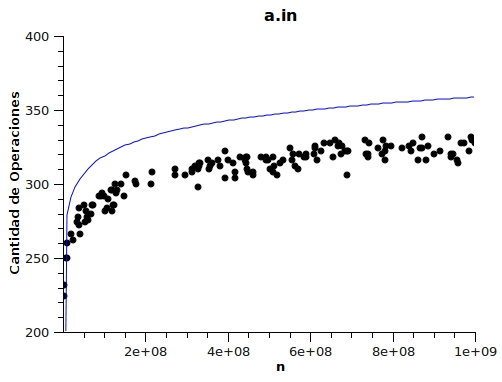
\includegraphics[scale = 0.8]{./../ej1/tests/a.jpg}
			\end{tabular}
			\caption{.} 
	\end{table}

	%grafico de b.in
	\begin{table}[ht]
		\centering 
			\begin{tabular}{c}
				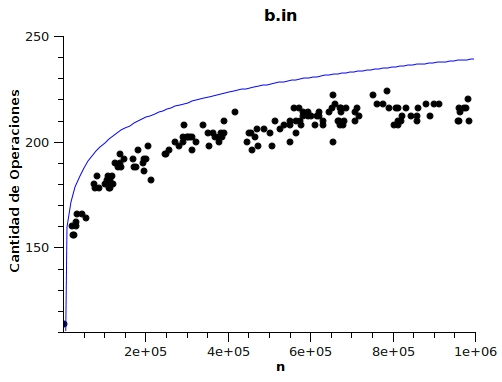
\includegraphics[scale = 0.8]{./../ej1/tests/b.jpg}
			\end{tabular}
			\caption{.} 
	\end{table}

	% grafico de c.in
	\begin{table}[ht]
		\centering 
			\begin{tabular}{c}
				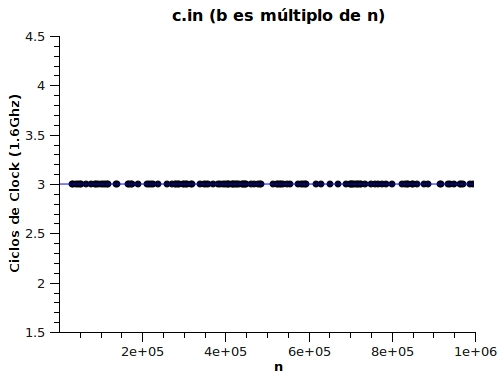
\includegraphics[scale = 0.8]{./../ej1/tests/c.jpg}
			\end{tabular}
			\caption{.} 
	\end{table}

	%grafico de d.in
	\begin{table}[ht]
		\centering 
			\begin{tabular}{c}
				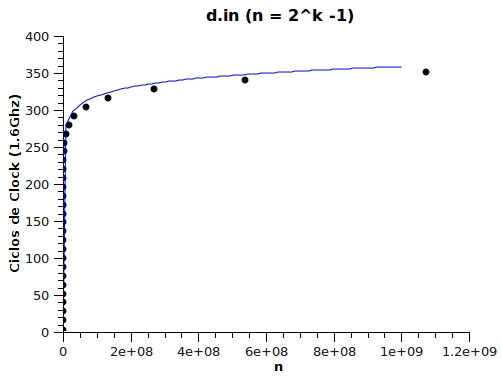
\includegraphics[scale = 0.8]{./../ej1/tests/d.jpg}
			\end{tabular}
			\caption{.} 
	\end{table}

	%grafico de e.in
	\begin{table}[ht]
		\centering 
			\begin{tabular}{c}
				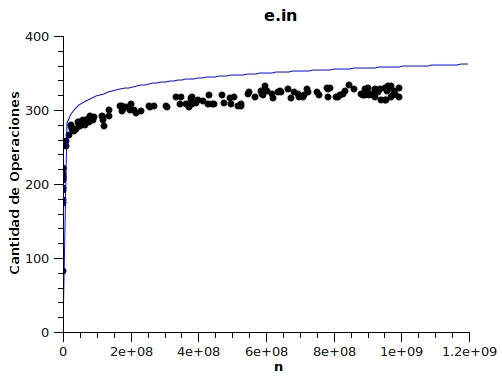
\includegraphics[scale = 0.8]{./../ej1/tests/e.jpg}
			\end{tabular}
			\caption{.} 
	\end{table}

	%grafico de f.in	
	\begin{table}[ht]
		\centering 
			\begin{tabular}{c}
				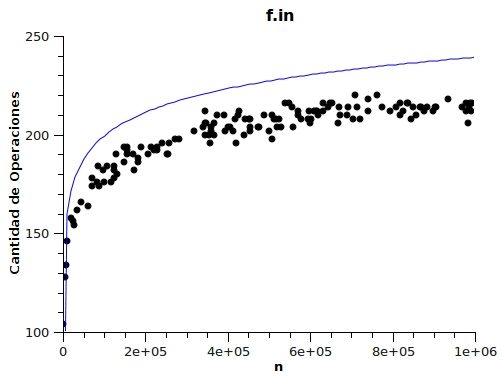
\includegraphics[scale = 0.8]{./../ej1/tests/f.jpg}
			\end{tabular}
			\caption{.} 
	\end{table}


%\subsection{Debate}
%\subsection{Comentarios}
%\subsection{Conclusiones}
